\chapter{Streamlining the development of parallel algorithms using Noarr}

% - many scientific algorithms are centered around a master data structure
%   - examples (matmul, transposition, physicell, ...)
% - the optimal run of these algorithms require an efficient memory traversal over the master data structure (both memory layout and traversal order) (both parallel and serial)
% - the domain experts usually can guess the optimal / close to optimal layout and traversal order
% - however, some optimizations require complex traversals that are very complex and error-prone to implement (tiling, levenstein, ...)
% - moreover, some traversting constants require tuning for different hardware (atlas)
% - other example is of a non expert who wants to speed up code by optimizing traversal - examples?
%   - there exist some dsls that can help with this
% - making this all by hand is very error-prone and time-consuming, unmantainable

% others do it too: cute, Kokos

% paper 1:
% - layout definition
% - allocation decoupling
% - layout agnostic
% - CUDA compatible
% - constants expressions
% - no overhead

% paper 2:
% - traversal definition / agnosticism
% - parallelism

Commonly, the core computation of scientific algorithms is centered around a master data structure. The examples include a matrix composed of cell features in an agent-based simulator~\cite{ghaffarizadeh2018physicell}, a grid of substrates in a diffusion solver~\cite{ghaffarizadeh2016biofvm}, a transition rates graph for Markov processes~\cite{koltai2020exact} \dots. In vast majority of these algorithms, the most performance-critical part hides in a nested loop over these data structures.

Possibly due to the lack of hardware expertise, there was no special attention paid to the memory performance when such loops were written~\cite{clauss2000automatic}. As a result, the programs show poor data locality, spending most of CPU cycles waiting for memory pipeline to deliver the data. It has been a result of many works, that changing the way how data is layed in memory of modifying the nested loops can result in a significant performance improvement~\cite{gong2018empirical,stengel2015quantifying,serpa2019memory}. Such optimizations may include decreasing the number of cache misses by grouping the operation on the same data together, employing prefetching by streamlining the memory access pattern or utilizing the vector instructions by aligning the data in memory.

Arguably, given a nested loop to optimize, the expert in performance optimization domain can pinpoint the biggest bottlenecks w.r.t. memory and propose close to optimal modifications with great probability. The most common modifications would include reordering the loops for the most possible serial access pattern and dividing the loops into tiles or strides to employ cache hierarchies~\cite{wolf1991data}. The issue, which takes the most programmers time, is putting these modifications into code. A simple tiling modification of nested loop of depth 3 already results in a verbose and error-prone code:
\begin{minted}[fontsize=\footnotesize,breaklines]{c++}
for (i = 0; i < I / 32; i++)
    for (j = 0; j < J / 32; j++)
        for (k = 0; k < K / 32; k++)
            for (ii = 0; ii < 32; ii++)
                for (jj = 0; jj < 32; jj++)
                    for (kk = 0; kk < 32; kk++)
\end{minted}

Many tools have been developed to alleviate this issue. Some provide automatic optimizations build within a compiler~\cite{trifunovic2010graphite,grosser2012polly}, some extend a compiler with annotations to guide the optimization process~\cite{donadio2005language,yi2007poet,chen2008chill,namjoshi2016loopy} and others include ad-hoc solutions for a specific family of algorithms~\cite{9485033,AFANASYEV2021100707}. However, a very little attention has been paid to aiding HPC programmers in writing the optimized code from the scratch, by providing them a clean and mantainable way to express complex loop traversal and memory layout fit for their specific problem.

To alleviate and streamline the mundane programming tasks repeatedly encountered during our work on optimizing scientific algorithms, we focused our work on developing a C++ library \emph{Noarr}. The main benefit of the library is that it allows to expressively and extensively define memory layouts of regular $n$-dimensional arrays and provides loop transformation primitives for their optimal traversal. It empowers HPC experts to swiftly develop their optimizations as a clean, error-prone code open to autotuning and parallelism, while staying within borders of a C++ standard without adding any dependency on the final software product (which is an advantage for the deployment in a scientific community).

% Arguably, the biggest requirement for the optimal performance of these algorithms is such traversal over the master data structure that generates memory accesses in the most hardware-efficient way. This can either mean: the least number of cache misses, the best utilization of the memory hierarchy, loop unrolling, automatized vectorization. To have a brief perspective on the importance, a simple matrix transposition runs 50x faster when traverzing data in the right order.  

% Critically, the expert int the performance optimization domain can usually guess the optimal or close to optimal traversal. In a big majority of cases, the proper cache utilization is just a question of iterating the loops in the right order and data tiling. The issue, which takes the most programmers time and is the most error-prone, is putting these traverals into code. A simple example of writing a tiling loop of 3D grid already results in an index hell.

% Furthermore, some optimizations require tuning of their parameters to be most efficient on a given hardware. For memory optimizations, such tunable parameters would be for example a size of a tile to fit given cache, or loop unrolling factor to sattisty the width of vector memory/compute instructions. Carrying out these tasks not in an automatized way is unmantainable and time-consuming. There are whole projects targeting automatic optimizations of specific algorithms, such as atlas for matrix multiplcation, FFTW for FFT, SPIRAL for signal processing. cuTLASS for CUDA matrix multiplication

% To alleviate and streamline these mundane programming tasks, which we encountered during our work on optimizing scientific algorithms multiple times, we focused our work here and developed a pure C++ library Noarr. Naturally, there are other libraries that aim to solve the same problem, the added value of noarr is:
% \begin{itemize}
%   \item a pure c++ approach without any need for DLS or precompilers. It empowers HPC experts to swiftly code their optimizations error-prone without adding any dependency on the final product. Which is usually paid huge attention to in a scientific community.
%   \item allows for simple tuning of the traversal constants for different hardware
%   \item CUDA compatible
%   \item support for parallelization of the traversal
%   \item %take sth from cgo paper
% \end{itemize}


\section{memory layouts and their traversal}

% - example of layout definition

% - example of traversal
% - how hard to define traversal by hand

% The main goal of noarr is to epressively and extensively define memory layouts and their traversals. There exists 

% definition of layout
% definition of traversal
% they are isomorphic, but layout can be stronger than traversal eg thanks to vector instructions
% there are not many libraries that allow to easily define custom layout.
% there are some, which do just a specific use cases, such as Kokkos (which is a big library and is specialized just on a set of specific use cases) GridTools similarly
% but recently, in parallel with our research, bigger players started to realize the importance of memory layout. ndspan in c++ standard and cute in cuda. ndspan is a good start, but noarr is much more extensible. cute was developed for Atlas, but it is not as general as noarr.
% noarr defines layout by composing atom protostructs
% column major, row major example in double for loop
% perhaps example of transformation c->r
% we require traversal to do it effectively
% for traversals, there are way more other tools that do the same. some of them do it automatically, polly. many of them are, however, annotation based, requiring custom compiler to precompile the code. or compiler pragmas. They target a different audience. similar comparison is openMP vs tbb. https://link.springer.com/content/pdf/10.1007/978-3-642-03869-3_62.pdf While TBB appears to be less appropriate for parallelizing existing implementations, it fosters a good programming style and higher abstraction level for newly developed parallel programs.
% show noarr traverse - some split tile example ... perhaps physicell

Generally, a way how data is layed in memory, a \emph{memory layout}, can be portrayed as a projection of its index space to a linear memory space. If we limit ourselves to a general (non-ragged) $n$-dimensional array, we can define memory layout mathematically as follows:

\begin{defn}[Memory Layout]
  Suppose a regular $n$-dimensional array $A$ with dimension lengths $d_1, \dots, d_n$ and an index space $\mathcal{I} = \{0,\dots,d_1 - 1\}\times \dots \times \{0,\dots,d_n - 1\}$. We define a \emph{memory layout} $\mathbb{L}$ of $A$ as a bijection $\mathbb{L}: \mathcal{I} \to \{0,\dots, \prod_{i}d_i - 1\}$. 
\end{defn}

Perhaps the most common memory layouts are row-major and column-major of a matrix. Their respective bijections can be generated by indexing functions $L_{\text{row}}(i,j) = i \cdot d_2 + j$ and $L_{\text{col}}(i,j) = j \cdot d_1 + i$ and these functions would be carried to source code with a slight modifications. 

As alluded to in the motivation, common layouts used to optimize memory accesses require a complex code. A tiled matrix layout, the layout paramount for some algorithms to optimally use cache hierarchies, already requires a verbose indexing function. Helping ourselves with adding two intra-tile dimensions, the indexing function would look as follows:
$$L_{\text{tiled}}(i,j,k,l) = (((i \cdot d_2 + j) \cdot d_3) + k) \cdot d_4 + l$$
Arguably, adding another tile dimension (to utilize multiple levels of cache) or swaping intra-tile layout to column-major form becomes less and less trivial. Considering the indexing functions are written ad-hoc, the layouts are tough subjects to change since a layout change reqires a thoughtful and error-prone rewrite of all index function occurences. Moreover, a complex indexing function is far from self-describing, making it hard, even close to impossible to guess the layouting intentions.

\subsection{Background}

The importance of these issues has been recognized by the HPC community, especially by the authors of HPC programming frameworks. Perhaps the oldest example is Kokkos~\cite{CARTEREDWARDS20143202}, a platform-agnostic programming model, that first defined a memory layout as a first class object. The layout is defined as a vector of dynamic dimension lengths; the dimensions are layed out in memory from left to right (leftmost dimension being layed in the memory continuously with a stride of 1, also called Fortran-style), from right to left (C-style) or by a custom vector of strides. Such simple approach covers a wide range of HPC use-cases and has been adopted by other frameworks, such as GridTools~\cite{AFANASYEV2021100707}.

Recently, more mainstream communities started to invest time. C++ has standardized mdspan in C++23. It takes a finer approach, allowing to define layout dimensions using a more complex extent structure.  Such structure allows to define some dimension lengths as static (known at compile time) and mix them with some dynamic (known at runtime). With such information during compile-time, a compiler can employ optimizations such as constant folding, loop unrolling or automatized vectorization. Similalry as with Kokkos, it also defines a LayoutPolicy, responsible for converting dimensions to underlying 1D memory. 



The developers familiar with this issue by encapsulating the memory layout into a complete object representing a data structure. Kokkos, platform-agnostic programming model, provides a simple syntax to define a list of static or dynamic dimensions of a multi-dimensional regular array and allows user to specify if the dimensions should be layed in memory from left to right (C-style), from right to left (Fortran-style) or in a custom stride.
GridTools provides a similar functionality, but it is more focused on the stencil computations and allows to select back-ends (GPU, multicore-CPU, \dots) according to which the most suitable layout will be selected. However, the memory layout is a very general concept and it is impossible to cover all the use-cases.

The mentioned works are mainly focused on a generalized optimization of a specific set of algorithms. They implement ways to efficiently parallelize problems, distribute and aggregate data. Still, they discovered that memory layout is integral part of the optimization process. Hence, they integrated some freedom of layout selection as a part of their libraries.

Standalone layouting stuff:
In parallel with our research, other works have been done in this area. C++ standard introduces mdspan, which will provide basic layouting functionality in standard library as soon as C++23 with more coming C++26. NVIDIA also realised the importance of extensive layouts and introduced CuTe library with a simmilar layouting algebra.
%https://arxiv.org/html/2312.11918v1/#S3

Noarr puts the biggest emphasis on expressiveness, perforamnce and extensibility of memory layouts. It is a standalone C++ header-only library based on template metaprogramming and is based on these principles:
\begin{itemize}
  \item \emph{named dimensions} The dimensions are not defined just by an order of some numbers, but they are named. This allows to query info of a dimension regardles its global index.
  \item \emph{trivial layouts} A set of trivial layout transformers is provided to allow to easily define complex layouts by composition of simple transformations.
\end{itemize}

Noarr borrows trivial tranformations from a well-known set of loop transformation, but extends it with some more. These are dimension reordering, 
strip mining, fusion, fission, but also a z-curve

Let us give an example of row-major matrix memory layout using noarr. Considering \mintinline{c++}{'i'} as a row dimension and \mintinline{c++}{'j'} as a column dimension, the layout can be defined as follows:
\begin{minted}[breaklines]{c++}
auto row_major = scalar<float>() ^ sized_vector<'j'>(n) ^ sized_vector<'i'>(m);
\end{minted}
The layout reads from left to right, signaling the innermost dimension first. 
It is apparent, that \mintinline{c++}{row_major} object represents only a layout, and to access the data, a memory pointer has to be provided:
\begin{minted}[breaklines]{c++}
float* data = new float[n * m];
float element = row_major | get_at<'i', 'j'>(data, 0, 0);
\end{minted}
To define a column-major layout, preserving the semantics of the dimension name, the layout can be defined as follows:
\begin{minted}[breaklines]{c++}
auto col_major = scalar<float>() ^ sized_vector<'i'>(m) ^ sized_vector<'j'>(n);
\end{minted}
The layout can be modified even more by introducing multiple dimensions. For example, to define a tiled layout, we add two more dimensions for the tiles:
\begin{minted}[breaklines]{c++}
auto tiled = scalar<float>() ^ sized_vector<'l'>(tile_n) ^ sized_vector<'k'>(tile_m) ^ sized_vector<'j'>(n / tile_n) ^ sized_vector<'i'>(m / tile_m);
\end{minted}
Here shows the power of named dimensions. Physically (in memory), \mintinline{c++}{'l'} and \mintinline{c++}{'k'} dimensions are innermost, representing column and row of a tile respetively. Dimensions \mintinline{c++}{'j'} and \mintinline{c++}{'i'} are outermost, representing column and row of a matrix, whose elements are whole tiles. With such semantics, tiles are both among themselves and within in row-major format. Unsurprisingly, the inter-tile layout can be changed to column-major by a simple rewrite: 
\begin{minted}[breaklines]{c++}
  auto tiled = scalar<float>() ^ sized_vector<'k'>(tile_m) ^ sized_vector<'l'>(tile_n) ^ sized_vector<'j'>(n / tile_n) ^ sized_vector<'i'>(m / tile_m);
\end{minted}


\subsection{Traversal}

As a complement to how memory is layed out, the way how it is traversed is equally important. A traversal over a data structure specifies an order, in which the elements of a data structure is accessed. Imagining such ordering as a bijection $\N \to \mathbb{I}$, where $\mathbb{I}$ is an index space of a data structure, the traversal shares many similarities with the memory layout. They both are subject to the same transformation: reordering, striping, tiling, \dots. With this in mind, it is easy to think that the aims of temporal locality and space locality are equaly achievable by both due to their isomorphic nature. https://dl.acm.org/doi/pdf/10.1145/346023.346031
Loop transformations are constrained by data dependencies, which may prohibit them from either coalesced memory loading on GPUs or vector instructions on CPUs. Nevertheless, traversal optimization is still a well reseached topic and complements the memory layout optimization especially when traversing multiple data structures of different layout at once, what is very common case.

Quantitatively, Loop transformation is perhaps more researched topic. Many approaches were explored. 

An automatized approach based on polyhedral models Polly, Graphite.

Annotation based tools.

Their extension to autotuning.


Our approach represents loop transformations as first class objects, which can be composed to form a complex transformation. Moreover, the loop transformation can be extended as a logical view over a memory layout. Let us revisit the example of tiling from the previous section. To traverse a matrix in tiles, we can define a traversal as follows:
A difference between layout and traversal is that traversal is represented as a set of nested loops. Let us have a simple example of copying data from row-major layout to a column-major layout. The naive loop would look like this: 
\begin{minted}[breaklines]{c++}
for (int i = 0; i < m; i++) {
  for (int j = 0; j < n; j++) {   
    column_major | get_at<'i', 'j'>(data, i, j) = row_major | get_at<'i', 'j'>(data, i, j);
  }
}
\end{minted}
However, such loop is not optimal. Cache misses are generated by the innermost loop, which is not cache-friendly. To optimize the loop, one can perform tiling:
\begin{minted}[breaklines]{c++}
for (int i = 0; i < m / tile_m; i ++) {
  for (int j = 0; j < n / tile_n; j ++) {
    for (int k = 0; k < tile_m; k ++) {
      for (int l = 0; l < tile_n; l ++) {
        column_major | get_at<'i', 'j'>(data, i * tile_m + k, j * tile_n + l) = row_major | get_at<'i', 'j'>(data, i * tile_m + k, j * tile_n + l);
      }
    }
  }
}
\end{minted}
This is not very readable and error-prone. Noarr provides a way to define such traversal in a more readable way:
\begin{minted}[breaklines]{c++}
traverser(tile_m, tile_n)
  .order(strip_mine<'i', 'i', 'k'>(tile_m) ^ strip_mine<'j', 'j', 'l'>(tile_n))
  .for_each([=](auto state)
  {
    column_major | get_at(data, state) 
      = row_major | get_at(data, state);
  });
\end{minted}
Here shows the power of named dimensions. The \mintinline{c++}{'i'} and \mintinline{c++}{'j'} dimensions are innermost, representing the column and row of a tile respectively. The \mintinline{c++}{'k'} and \mintinline{c++}{'l'} dimensions are outermost, representing the column and row of a matrix, whose elements are whole tiles. With such semantics, tiles are both among themselves and within in row-major format. Unsurprisingly, the inter-tile layout can be changed to column-major by a simple rewrite:

There are other transformations \dots



\subsection{layout agnostic code}

Benefits of some annotation-based tools is the ability to automatically search transformation space and find the most optimal traversal. Such \emph{autotuning} is especially useful when the code is supposed to run on different hardware. The different cache sizes or vector registers widths can be easily adapted to by the autotuning process.

As first-class objects, noarr layouts and traversals allow for \emph{layout-agnostic} and \emph{traversal-agnostic} code. A code, which contains the performance critical part, such as nested for loop of a scientific algorithm, can be encapsulated in a function, with traversal and layout extracted into function parameters:
\begin{listing}
  \begin{minted}[fontsize=\footnotesize,linenos,breaklines]{c++}
  template <class A_t, class B_t, class C_t, class Order_t>
  void matmul(A_t& A, B_t& B, C_t& C, Order_t my_order) 
  {
      traverser(A, B, C).order(my_order).for_each([&](auto Aidxs, auto Bidxs, auto Cidxs)
      {
          C.at(Cidxs) += A.at(Aidxs) * B.at(Bidxs);
      });
  }
  \end{minted}
  \caption{Traversal-agnostic matrix multiplication}
  \label{lst:agn}
\end{listing}

The function can be called repeatedly with a different combination of layout and traversal transformations. Benchmarking the differently parametrized functions then shows the optimal transformations on a running hardware and highlights the most effective optimizations on a general hardware.

% add figure heatmap_all

\begin{figure}
  \centering
  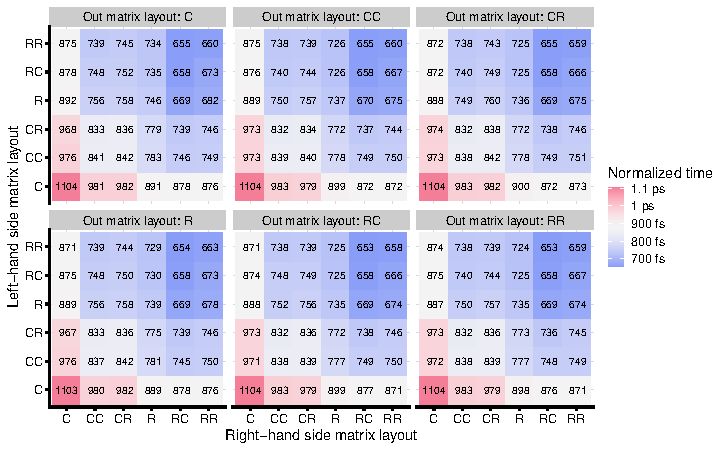
\includegraphics[width=0.8\textwidth]{img/heatmap_all}
  \caption{Heatmap of the execution time of a matrix multiplication algorithm with different layout and traversal transformations. The optimal transformation is highlighted in red.}
  \label{fig:heatmap_all}
\end{figure}

The modular template-based design of this extension al-
lows us to mimic the autotuning systems, which search the
vast space of transformation, trying to find the most per-
formant one for a specific computational function. In our
approach, we may be able to express precisely that with
so-called traversal-agnostic functions — the body of such
functions does not change, although the traversal order does
(see Listing 7).

Our approach may promote less time spent in code compiling as we do not require to modify the source code when applying the different transformations. However, this is farfrom the scope of this paper.

% benefits of some of annotation based tools is the ability to autotune some layout parameters
% noarr layout agnostic abstraction allows just the same
% example of layout agnostic
% code can run irrespective the traversal used (assuming the traversal is correct)(isomorphic)
% find sth from cgo paper


\section{parallelism}

% parallelism is a different kind of beast, it can alter the traversal
% considering algorithms with master data structures, the parallelism is usually a question of in which nested loop are we aiming to parallelize
% there can be caveats ofcourse, such as data dependencies, but they are usually easy to spot
% there can be caveats, such as different hierarchies of parallelsim (either be it simd on CPUs or more prevalent GPU) - so there is a need to divide in multiple levels
% noarr traversals are general enough to do this in a custom way
% nevetherless, we experimented with wrappers around tbb to provide proof of concept
% wrapper around cuda kernel launch which divides over 2 dims
% structure for cuda shared mem?
% examples



